\documentclass{article}

\usepackage[utf8]{inputenc}
\usepackage{amsmath}
\usepackage{amssymb}
\usepackage{anysize}
\usepackage{color}
\usepackage{xcolor}
\usepackage{graphicx}

\usepackage{listings}
\lstset{
	language=C++,                	% choose the language of the code
	basicstyle=\footnotesize,       % the size of the fonts that are used for the code
	numbers= left,                 	% where to put the line-numbers
	numberstyle=\footnotesize,      % the size of the fonts that are used for the line-numbers
	stepnumber=1,                   % the step between two line-numbers. If it is 1 each line will be numbered
	numbersep=5pt,                  % how far the line-numbers are from the code
	backgroundcolor=\color{white},  % choose the background color. You must add \usepackage{color}
	showspaces=false,               % show spaces adding particular underscores
	showstringspaces=false,         % underline spaces within strings
	showtabs=false,                 % show tabs within strings adding particular underscores
	frame=single,           		% adds a frame around the code
	tabsize=2,          			% sets default tabsize to 2 spaces
	captionpos=t,          			% sets the caption-position to bottom (t=top, b=bottom)
	breaklines=true,        		% sets automatic line breaking
	breakatwhitespace=false,    	% sets if automatic breaks should only happen at whitespace
	escapeinside={\%*}{*)}          % if you want to add a comment within your code
}



\usepackage{caption}
\DeclareCaptionFont{white}{\color{white}}
\DeclareCaptionFormat{listing}{\colorbox{gray}{\parbox[c]{\textwidth}{#1#2#3}}}
\captionsetup[lstlisting]{format=listing,labelfont=white,textfont=white}

\setlength\parindent{0pt}
\setlength{\parskip}{10pt}

\marginsize{3cm}{2cm}{2cm}{2cm}

\title{Software Engineering\\
		Lab 4 Report}
\author{Emre Ozan Alkan\\
		\{emreozanalkan@gmail.com\}\\
		MSCV-5}
\date{1 November 2013}

\begin{document}
\maketitle

\section{2D Point}

	\subsection{Declare and implement Point2d class}

\begin{lstlisting}[label=Point2d,caption=Point2d.h]	
#ifndef POINT2D_H
#define POINT2D_H

#include <iostream>

// Representing 2D point
// 2 points represented by float values x and y
// Has pointers to previous and next elements
// to be used in chain list data structure
class Point2d
{
private:
    // Represents the value of x coordinate of 2D point
    float _x;
    // Represents the value of y coordinate of 2D point
    float _y;

    // Keeps track of the previous element in chain list
    Point2d* _prev;
    // Keeps track of the next element in chain list
    Point2d* _next;
public:
    // Default Constructor
    Point2d();
    // Overloaded Constructor for initializing values _x and _y
    Point2d(float, float);
    // Deconstructor
    ~Point2d();

    // Displays the values of _x, _y
    // and addresses of the _prev and _next pointers
    void display() const;

    // Setter of _x
    void setX(float);
    // Getter of _x
    float getX() const;

    // Setter of _y
    void setY(float);
    // Getter of _y
    float getY() const;

    // Setter of _prev
    void setPrev(Point2d*);
    // Getter of _prev
    Point2d* getPrev() const;

    // Setter of _next
    void setNext(Point2d*);
    // Getter of _next
    Point2d* getNext() const;

    // Sets the value of _x and _y
    void set(float, float);
    // Sets the value of _x and _y with given another point by pointer
    void set(const Point2d*);
    // Sets the value of _x and _y with given another point by reference
    void set(const Point2d&);

    // Asks user to get _x and _y values
    void askvalue();
};

#endif // POINT2D_H
\end{lstlisting}


		\subsection{Implement member function display(...) and operator overload}
		
\begin{lstlisting}[label=point2d-display,caption=Point2d::display()]	
void Point2d::display() const
{
    std::cout<<"POINT x:"<<_x<<" y:"<<_y;
    std::cout<<" P:"<<std::hex<<_prev;
    std::cout<<" N:"<<std::hex<<_next;
    std::cout<<std::endl;
}

std::ostream& operator<<(std::ostream& os, const Point2d& point)
{
  point.display();
  return os;
}

std::ostream& operator<<(std::ostream& os, const Point2d* point)
{
  point->display();
  return os;
}

\end{lstlisting}

		\subsection{Setters, Getters and askvalue(...)}
		
\begin{lstlisting}[label=setters-getters,caption=Setters-Getters]	
void Point2d::setX(float x)
{
    _x = x;
}

float Point2d::getX() const
{
    return _x;
}

void Point2d::setY(float y)
{
    _y = y;
}

float Point2d::getY() const
{
    return _y;
}

void Point2d::set(float x, float y)
{
    _x = x;
    _y = y;
}

void Point2d::set(const Point2d* point)
{
    this->_x = point->getX();
    this->_y = point->getY();
}

void Point2d::set(const Point2d& point)
{
    this->_x = point.getX();
    this->_y = point.getY();
}

void Point2d::askvalue()
{
    std::cout<<"x?";
    std::cin>>_x;
    std::cout<<"y?";
    std::cin>>_y;
}

\end{lstlisting}



		\subsection{Declare and Initialize a dummy Point2d}
		
\begin{lstlisting}[label=dummy-point2d,caption=Dummy Test]	
int main(int argc, char *argv[])
{
    cout<<"Point2d Dummy Test"<<endl;
    cout<<"------------------"<<endl;
    Point2d *dummy = new Point2d();

    dummy->display();
    dummy->set(.4, 5.);
    dummy->display();
    dummy->setX(3.8);
    dummy->setY(1.2);
    dummy->display();
    dummy->askvalue();
    cout<<dummy;

    delete dummy;
    dummy = 0;
    return 0;
 }
\end{lstlisting}






\section{Polygon}

\begin{figure}[ht!]
\centering
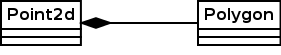
\includegraphics{Diagram1.png}
\caption{Polygon compose of Point2ds}
% \label{overflow}
\end{figure}


	\subsection{Declare and implement Polygon class}
\begin{lstlisting}[label=Polygon,caption=Polygon.h]	
#ifndef POLYGON_H
#define POLYGON_H

#include "Point2d.h"

// Representing a polygon with 2D points
// Polygon class compose of Point2d classes
// Polygon class keeps root of the chain list
// represented with Point2d pointer: _start
class Polygon
{
private:
    // Representing the first element in the double chained list
    Point2d* _start;
public:
    // Default constructor
    Polygon();
    // Desctructor
    ~Polygon();

    // Displays the indexes, addresses of the elements in chain list
    // and displays Point2d itself
    void display() const;

    // Setter of the _start
    void setStartPoint(Point2d*);
    // Getter of the _start
    Point2d* getStartPoint() const;

    // Returns the first element in chain list: _start
    Point2d* begin() const;
    // Returns the size of the double chain list
    int size() const;
    // Returns the item in the given index
    Point2d* get_item(int) const;
    // Inserts the given item with pointer to the end of the chain list
    void insert(Point2d*);
    // Inserts the given item with pointer to the given index, otherwise end of the chain list
    void insert_at(Point2d*, int = -1);
    // Deletes the item from the given index
    void delete_at(int);

    // [] operator overload returns the item specified with index
    Point2d* operator[](int);

    // Creates new polygon and returns its pointer
    static Polygon* BuildPolygon();
    // Creates new polygon, creates number of Point2d elements specified with parameter
    // Ask user for values of the points and returns the created polygon's pointer
    static Polygon* BuildPolygon(int);
    // Creates number of Point2d elements specified with parameters and asks user their values
    // and assign them to the given polygon by pointer
    static void BuildPolygon(Polygon*, int);
    // Creates number of Point2d elements specified with parameters and asks user their values
    // and assign them to the given polygon by reference
    static void BuildPolygon(Polygon&, int);
};

#endif // POLYGON_H
\end{lstlisting}

		\subsection{Declare and Implement BuildPolygon(...) function}
		
\begin{lstlisting}[label=buildpolygon,caption=BuildPolygon()]	
Polygon* Polygon::BuildPolygon()
{
    return new Polygon();
}

Polygon* Polygon::BuildPolygon(int nPoints)
{
    Polygon* polygon = new Polygon();

    for(int i = 0; i < nPoints; i++)
    {
        Point2d* point = new Point2d();

        point->askvalue();

        polygon->insert(point);
    }

    return polygon;
}

void Polygon::BuildPolygon(Polygon* polygon, int nPoints)
{
    if(!polygon)
        polygon = Polygon::BuildPolygon();

    for(int i = 0; i < nPoints; i++)
    {
        Point2d* point = new Point2d();

        point->askvalue();

        polygon->insert(point);
    }
}

void Polygon::BuildPolygon(Polygon& polygon, int nPoints)
{
    for(int i = 0; i < nPoints; i++)
    {
        Point2d* point = new Point2d();

        point->askvalue();

        polygon.insert(point);
    }
}

\end{lstlisting}


		\subsection{Declare and Implement function that displays elements of polygon}
		
\begin{lstlisting}[label=polygon-display,caption=Polygon::display()]	
void Polygon::display() const
{
    std::cout<<"Polygon:"<<std::endl;

    for(int i = 0; i < this->size(); i++)
    {
        Point2d *point = this->get_item(i);
        std::cout<<"index:"<<i<<" addr:"<<std::hex<<point<<std::endl;
        point->display();
        point = 0;
    }
}

std::ostream& operator<<(std::ostream& os, const Polygon& polygon)
{
  polygon.display();
  return os;
}

std::ostream& operator<<(std::ostream& os, const Polygon* polygon)
{
  polygon->display();
  return os;
}

\end{lstlisting}








\section{Insertion and deletion of elements}
Here is the section for double chained list data structure functions implemented.


		\subsection{begin() that returns a pointer to the first element}
		
\begin{lstlisting}[label=polygon-begin,caption=Polygon::begin() const]	
Point2d* Polygon::begin() const
{
    return _start;
}

\end{lstlisting}

		\subsection{size() that returns the number of points in the polygon}
		
\begin{lstlisting}[label=polygon-size,caption=Polygon::size() const]	
int Polygon::size() const
{
    int size = 0;

    Point2d* temp = this->begin();

    if(!temp) return 0;

    do
    {
        size++;
        temp = temp->getNext();
    }while(temp != this->begin());

    return size;
}

\end{lstlisting}

		\subsection{getitem() that returns a pointer to a 2D Point at position in a given polygon}
		
\begin{lstlisting}[label=polygon-getitem,caption=Polygon::getitem(int) const]	
Point2d* Polygon::get_item(int index) const
{
    if(index >= this->size())
    {
        std::cerr<<"get_item(): Index out of range at index:"<<index<<" size was:"<<this->size()<<std::endl;
        return 0;
    }

    Point2d* temp = this->begin();

    for(int i = 0; i < index; i++)
        temp = temp->getNext();

    return temp;
}

\end{lstlisting}

		\subsection{insertat() that inserts an element at a given position in the list}
		
\begin{lstlisting}[label=polygon-insert,caption=Polygon::insertat(int)]	
void Polygon::insert(Point2d* point)
{
    Point2d* temp = this->begin();

    if(!temp)
    {
        this->setStartPoint(point);
        point->setNext(point);
        point->setPrev(point);
        return;
    }

    while(temp->getNext() != this->begin())
        temp = temp->getNext();

    point->setPrev(temp);
    point->setNext(this->begin());
    temp->setNext(point);
    this->begin()->setPrev(point);
}

void Polygon::insert_at(Point2d* point, int index)
{
    if(index == -1)
        this->insert(point);

    int size = this->size();

    if(index > size || index < 0)
    {
        std::cerr<<"insert_at(): Index out of range at index:"<<index<<" size was:"<<this->size()<<" to "<<point<<std::endl;
        return;
    }
    if(index == size)
        this->insert(point);


    Point2d* temp = this->get_item(index);

    point->setPrev(temp->getPrev());
    point->setNext(temp);
    temp->getPrev()->setNext(point);
    temp->setPrev(point);
}

\end{lstlisting}

		\subsection{deleteat() that deletes (if possible) an element at given position}
		
\begin{lstlisting}[label=polygon-delete,caption=Polygon::deleteat(int)]	
void Polygon::delete_at(int index)
{
    if(index >= this->size())
    {
        std::cerr<<"delete_at(): Index out of range at index:"<<index<<" size was:"<<this->size()<<std::endl;
        return;
    }

    Point2d* temp = this->get_item(index);

    temp->getPrev()->setNext(temp->getNext());
    temp->getNext()->setPrev(temp->getPrev());

    delete temp;
}

\end{lstlisting}

		\subsection{Overload the operator [] for such class}
		
\begin{lstlisting}[label=polygon-index_operator,caption=Polygon::operator[](int)]	
Point2d* Polygon::operator[](int index)
{
    if(index >= this->size())
    {
        std::cerr<<"operator[](): Index out of range at index:"<<index<<" size was:"<<this->size()<<std::endl;
        return 0;
    }

    Point2d* temp = this->get_item(index);

    return temp;
}

\end{lstlisting}




\section{Results}
Results I obtained

		\subsection{Example main}
		
\begin{lstlisting}[label=example-main,caption=main.cpp]	
int main(int argc, char *argv[])
{
    cout<<"Point2d Dummy Test"<<endl;
    cout<<"------------------"<<endl;
    Point2d *dummy = new Point2d();

    dummy->display();
    dummy->set(.4, 5.);
    dummy->display();
    dummy->setX(3.8);
    dummy->setY(1.2);
    dummy->display();
    dummy->askvalue();
    cout<<dummy;

    delete dummy;
    dummy = 0;

    cout<<endl<<endl;


    cout<<"Polygon Test"<<endl;
    cout<<"------------------"<<endl;

    Polygon* polygon = Polygon::BuildPolygon(4);

    polygon->display();

    cout<<"Current Size: "<<polygon->size()<<endl;

    Point2d* testPoint1 = new Point2d();
    testPoint1->askvalue();

    polygon->insert(testPoint1);

    cout<<"Current Size: "<<polygon->size()<<endl;

    polygon->display();

    Point2d* testPoint2 = new Point2d();
    testPoint2->askvalue();

    polygon->insert_at(testPoint2, 2);

    cout<<"Current Size: "<<polygon->size()<<endl;

    polygon->display();

    polygon->delete_at(2);

    cout<<"Current Size: "<<polygon->size()<<endl;

    cout<<polygon; //polygon->display();

    delete polygon;

    return EXIT_SUCCESS;
}

\end{lstlisting}


		\subsection{Example main}

\begin{figure}[ht!]
\centering
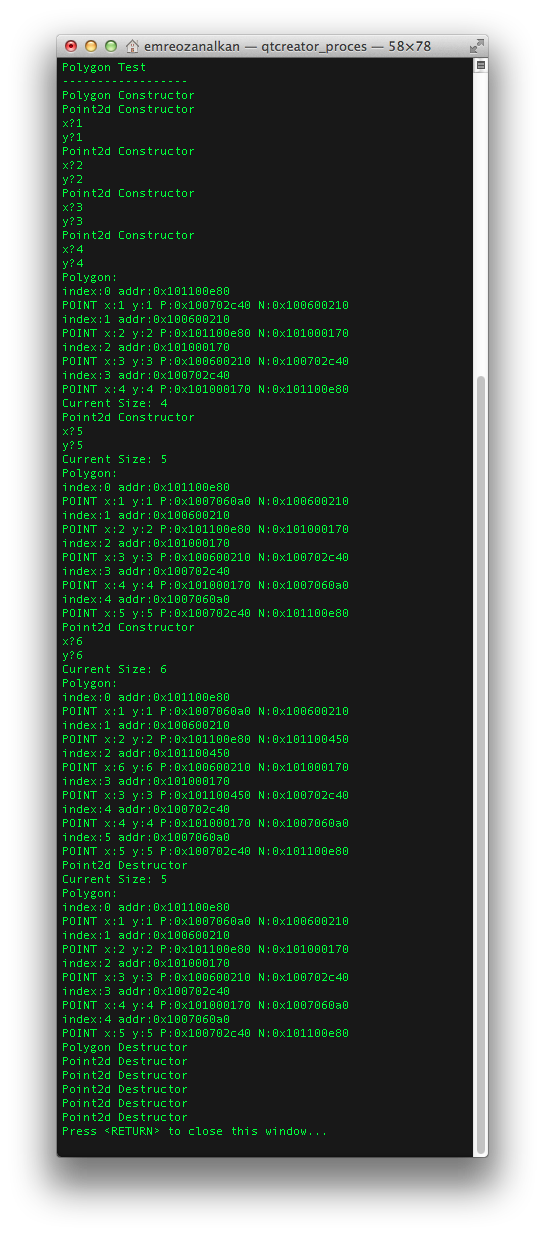
\includegraphics[height=280mm]{Output1.png}
\caption{Lab 4 - Output}
%\label{overflow}
\end{figure}




\end{document}







































